\documentclass[conference]{IEEEtran}
\usepackage{times}

% numbers option provides compact numerical references in the text.
\usepackage[numbers]{natbib}
\usepackage{multicol}
\usepackage[bookmarks=true]{hyperref}
\usepackage{amsmath,amssymb}
% \usepackage[standard]{ntheorem}
\usepackage{amsthm}
\usepackage{mathtools}
\usepackage{bm}
\usepackage{graphicx}
% \usepackage{caption}
% \usepackage{figure}
\usepackage{float}
\usepackage{subcaption}
\usepackage{epstopdf}
\usepackage{dblfloatfix}
\usepackage{fixltx2e}
% \usepackage{subfig}
\usepackage{mathrsfs}
\usepackage{algorithm}
\usepackage{algorithmicx}
\usepackage[noend]{algpseudocode}
\makeatletter
\def\BState{\State\hskip-\ALG@thistlm}
\makeatother
\algdef{SE}[DOWHILE]{Do}{DoWhile}[1]{\algorithmicdo\ #1}[1]{\algorithmicwhile\ #1}

\usepackage{booktabs}
\newcommand\Tstrut{\rule{0pt}{2.5ex}}       % "top" strut
\newcommand\Bstrut{\rule[-0.9ex]{0pt}{0pt}} % "bottom" strut
\newcommand{\TBstrut}{\Tstrut\Bstrut} % top&bottom struts

\usepackage{tabstackengine}
\stackMath

\usepackage{tikz}
\usetikzlibrary{scopes}
\usetikzlibrary{shapes.misc}
\tikzset{cross/.style={cross out, draw=black, minimum size=2*(#1-\pgflinewidth), inner sep=0pt, outer sep=0pt},
%default radius will be 1pt.
cross/.default={2pt}}

\let\labelindent\relax
\usepackage{enumitem}
% \newenvironment{enum}{\begin{enumerate}[wide, labelwidth=!, labelindent=0pt]}{\end{enumerate}}
\newlist{inparaenum}{enumerate}{2}% allow two levels of nesting in an enumerate-like environment
\setlist[inparaenum]{nosep,wide,labelwidth=!,labelindent=0pt}% compact spacing for all nesting levels
\setlist[inparaenum,1]{label=\bfseries\arabic*)}% labels for top level
\setlist[inparaenum,2]{label=\arabic{inparaenumi}{\alph*})}% labels for second level

\newtheorem{theorem}{Theorem}
\newtheorem{proposition}{Proposition}
\newtheorem{definition}{Definition}
\newtheorem{corollary}{Corollary}
\newcommand\numberthis{\addtocounter{equation}{1}\tag{\theequation}}
\DeclareMathOperator{\sign}{\text{sgn}}
\DeclareMathOperator*{\argmin}{arg\,min}
\DeclareMathOperator{\intr}{int}
\DeclareMathOperator{\dom}{dom}
\DeclareMathOperator{\rot}{\text{rot}}

\newcommand{\BB}[1]{{\color{red} {Byron: {#1}}}}

\newcommand{\EH}[1]{{\color{blue} {Eric: {#1}}  }}
\newcommand{\AB}[1]{{\color{cyan} {Ankit: {#1}}  }}
\newcommand{\TODO}[1]{{\color{red} {{#1}}  }}

\pdfinfo{
   /Author (Eric Huang)
   /Title  (Robots: Our new overlords)
   /CreationDate (D:20161016120000)
   /Subject (Robots)
   /Keywords (Robots;Overlords)
}

\begin{document}

% paper title
\title{\huge Exact Bounds on the Contact Driven Motion of a Sliding
  Object, With Applications to Robotic Pulling}

% You will get a Paper-ID when submitting a pdf file to the conference system
% \author{Author Names Omitted for Anonymous Review. Paper-ID [65]}

\author{\authorblockN{Eric Huang\authorrefmark{2},
Ankit Bhatia\authorrefmark{2},
Byron Boots\authorrefmark{1} and
Matt Mason\authorrefmark{2}}
\authorblockA{\authorrefmark{2}Robotics Institute\\
Carnegie Mellon University,
Pittsburgh, Pennsylvania 15213\\ Email: \{erich1,ankitb\}@andrew.cmu.edu, matt.mason@cs.cmu.edu}
\authorblockA{\authorrefmark{1}Interactive Computing\\
Georgia Institute of Technology,
Atlanta, Georgia 30332\\ Email: bboots@cc.gatech.edu}}

% \author{\authorblockN{Michael Shell}
% \authorblockA{School of Electrical and\\Computer Engineering\\
% Georgia Institute of Technology\\
% Atlanta, Georgia 30332--0250\\
% Email: mshell@ece.gatech.edu}
% \and
% \authorblockN{Homer Simpson}
% \authorblockA{Twentieth Century Fox\\
% Springfield, USA\\
% Email: homer@thesimpsons.com}
% \and
% \authorblockN{James Kirk\\ and Montgomery Scott}
% \authorblockA{Starfleet Academy\\
% San Francisco, California 96678-2391\\
% Telephone: (800) 555--1212\\
% Fax: (888) 555--1212}}

% avoiding spaces at the end of the author lines is not a problem with
% conference papers because we don't use \thanks or \IEEEmembership

% for over three affiliations, or if they all won't fit within the width
% of the page, use this alternative format:
% 
% \author{\authorblockN{Michael Shell\authorrefmark{1},
% Homer Simpson\authorrefmark{2},
% James Kirk\authorrefmark{3}, 
% Montgomery Scott\authorrefmark{3} and
% Eldon Tyrell\authorrefmark{4}}
% \authorblockA{\authorrefmark{1}School of Electrical and Computer Engineering\\
% Georgia Institute of Technology,
% Atlanta, Georgia 30332--0250\\ Email: mshell@ece.gatech.edu}
% \authorblockA{\authorrefmark{2}Twentieth Century Fox, Springfield, USA\\
% Email: homer@thesimpsons.com}
% \authorblockA{\authorrefmark{3}Starfleet Academy, San Francisco, California 96678-2391\\
% Telephone: (800) 555--1212, Fax: (888) 555--1212}
% \authorblockA{\authorrefmark{4}Tyrell Inc., 123 Replicant Street, Los Angeles, California 90210--4321}}

\maketitle

\begin{abstract}
  This paper explores the quasi-static motion of a planar slider being
  pushed or pulled through a single contact point assumed not to
  slip. The main contribution is to derive a method for computing
  exact bounds on the object's motion for classes of pressure
  distributions where the center of pressure is known but the
  distribution of support forces is unknown. The second contribution
  is to show that the exact motion bounds can be used to plan robotic
  pulling trajectories that guarantee convergence to the final
  pose. The planner was tested on the task of pulling an acrylic
  rectangle to random locations within the robot workspace. The
  generated plans were accurate to 4.00mm $\pm$ 3.02mm of the target
  position and 4.35 degrees $\pm$ 3.14 degrees of the target
  orientation.

  % \EH{TODO: Experimental results} 

  % The distance between the upper and lower motion bounds were 
  % 5-10$\times$ 

  % The exact bounds were shown to 

  % The exact motion bounds an tighter over wide range of object
  % geometries.

% Major contributions:
%   \begin{enumerate}
%   \item Proof of stability
%   \item first known algorithm that computes exact angular velocity
%     bounds on the friction dominated motion of a pushed/pulled object.
%   \item Uncertainty bounds on the orientation
%   \item Planner that exploits the stability of pulling using the exact
%     angular velocity bounds.
%   \item to return trajectories.
%   \item An easy to implement in both hardware and software skill. 
%   \item validated on a real robotic system.
%     A useful addition to a roboticist's toolkit. that is serviceable
%     in a wide range of scenarios. ranging from furniture rearrangement
%     or table-top manipulation to bin picking.
%   \end{enumerate}
\end{abstract}

\IEEEpeerreviewmaketitle

\section{Introduction}

% \TODO{
% Items that an introduction should address:
% \begin{enumerate}
% \item What is the problem?
% \item Why should people care?
% \item What are the major contributions?
% \item What is the structure of this paper?
% \end{enumerate}
% }

% In this paper, we demonstrate the value of 

% \begin{enumerate}
% \item Looking at pushing from a different perspective
% \item contributions
% \item open-loop stable with convergence guarantees
% \item easy to use
% \item Outline of sections
% \end{enumerate}

% \begin{inparaenum}
% \item 

Pushing (or pulling) planar objects with fixed contact is difficult to
model in both theory and practice. First, pressure distributions of
objects are statically indeterminant (barring the case of three-point
support with known center of mass). Second, surface imperfections lead
to spatial variability in both the pressure distribution and
coefficient of friction \cite{YuBFR16}. Though several force-motion
models for pushing exist
\cite{zhou2016convex,howe1996practical,goyal1991planar}, the above
sources of indeterminacy ultimately lead to errors in the predicted
velocity of the pushed object.

If the motion cannot be predicted, then another option is to find
bounds on the velocity of the pushed object. This problem was first
raised in Mason's thesis on robotic pushing \cite{Mason1982}. In the
case of fixed contact pushing, this is equivalent to finding bounds on
angular velocity of the object as it is pushed through the contact
point. To this end, we develop the first algorithm that finds
\textit{exact} angular velocity bounds on the object's motion over all
pressure distributions with shared center of pressure. Moreover, the
bounds are exact for many additional classes of pressure distributions
that have not been considered before.

Dealing with uncertainty is a fundamental challenge in robotics
\cite{Thrun2005}. We demonstrate how our bounds can be applied to
planning for robotic pulling under action uncertainty. Robotic pulling
is a general-purpose manipulation skill for positioning and orienting
objects. The proposed planner uses the angular velocity bounds to find
actions that reduce the uncertainty in the system, i.e. close the
distance between the integrated orientation bounds. Moreover, given a
suitable initialization, the planner finds trajectories that guarantee
the uncertainty at the final pose converges to a very small value.

The rest of the paper is organized as follows. Section
\ref{sec:related-work} discusses related work. Section
\ref{sec:background} summarizes the relevant background on planar
pushing needed to understand our work. Section \ref{sec:theory}
develops several theoretical results needed to prove the correctness
of our algorithmic contributions. Section \ref{sec:methods} introduces
the exact angular velocity bound algorithm and the algorithm for
planning pulling trajectories under action uncertainty. Section
\ref{sec:experiments} presents our experimental results. Section
\ref{sec:conclusion} gives concluding remarks on the paper.

% one reason for this success is because pulling has convenient
% stability properties. Barring the one unstable equilibrium point, an
% object pulled in a straight line converges to a stable equilibrium.

% The rationale for this is that, 

% there exists a stable and unstable equilibrium when

% Because stable equilibria 

% The end-product is 

% A subset of pulling trajectories are stable 

% Dragging objects 

% Because pulling is an inherently stable maneuver, 

% Our planner maintains bounds on the object pose during a
% trajectory and reasons \\

% where the robot contacts a rigid body at a point and pulls
% that contact point along a trajectory. 

% Pulling is especially useful for manipulating objects that are too
% large or heavy to be picked or objects that are tucked away and
% difficult to reach.

% We apply our bounds to planning under uncertainty.
% We verify 

% Uncertainty arises from many sources including limited
% sensors, incomplete models, and stochastic actions. In this work, we
% introduce robotic pulling as a method of robotic manipulation that
% remains stable in the presence of uncertainty.

% Robotic pulling is a general-purpose manipulation skill for positioning and
% orienting objects where the robot contacts a
% rigid body at a point and pulls that contact point along a
% trajectory. Pulling is especially useful for manipulating objects that are too
% large or heavy to be picked or objects that are tucked away and difficult
% to reach.

% In this paper, we introduce the theoretical and practical formulation
% of pulling as a primitive action for positioning and orienting objects
% under uncertainty. An important contribution of our approach is
% showing that, when pulling, %, even during open-loop control,
% the system uncertainty (error) remains Lyapunov
% stable. %Next, we highlight the results that enable us to create our primitive action planner for pulling.
%
%The insight that motivated this work was our recognition, and
%subsequent proof, of the stability of pulling. 
% Consider the following example: if an object is pulled
% in a straight line along a surface, the frictional forces cause the
% object to rotate around the contact point until the object's center of
% mass aligns with the line of motion. We show how algorithms can take advantage of
% this kind of stability to guarantee the object has been pulled into the
% correct position and orientation.

% To show the practical benefit of our approach, we use Differential Dynamic Programming (DDP) as a
% locally optimal planner for computing pulling trajectories. By
% augmenting the dynamics with the orientation bounds, we allow DDP to
% track the convergence of the pulled object. In Section~\ref{} we verify this approach 
% both in simulation and on a real robotic system.
% \end{inparaenum}

% \begin{inparaenum}
% \item Section \ref{sec:related-work}
% \item Section \ref{sec:theory}
% \item Section \ref{sec:methods}
% \item Section \ref{sec:experiments}
% \end{inparaenum}

% Stability alone is not a sufficient for planning with convergence
% guarantees. % to enable planning to guarantee convergence.
% A practical planner also requires knowledge of the object's rate of
% convergence to the stable configuration.

% Toward this end, we develop the first known algorithm that computes
% exact angular velocity bounds on the motion of a pushed or pulled
% object. The bounds can be made arbitrarily tight by specifying a
% convex set of candidate pressure distributions over which to compute
% them. In addition, we prove that the angular velocity bounds can be
% integrated into orientation bounds, which can be used for planning
% convergent trajectories.

% In contrast to the prior art, our algorithm is the first to find
% \textit{exact} angular velocity bounds for a pushed object. 

\section{Related Work}\label{sec:related-work}

% Mason's seminal thesis on robotic pushing \cite{Mason1982} was the
% first to raise the problem of bounding the motion of a pushed object
% as an alternative to the errors associated with exact models.
% The problem of bounding the motion 
% ``If the [motion] cannot be predicted, then the next best thing is to
% determine the range of possible [motions].''

% Prior work bounding the pushed motion of an object is largely
% organized by the bounds on object motion that can be obtained and the
% assumptions required.

We can categorize prior work bounding the motion of a pushed object
according to the tightness of the bounds and the basic assumptions
from which those bounds are deduced, such as knowledge of the center
of pressure location.
%
The bisector bound restricts the feasible rotation centers to a
half-space delimited by the perpendicular bisector between the contact
point and center of pressure \cite{Mason}.  Alexander and Maddocks
bounded the set of feasible rotation centers to lie within the minimum
object-enclosing vertical strip perpendicular to the wrench applied by
the pusher \cite{alexander1993bounds}.  Peshkin and Sanderson bounded
the motion of a pushed object by computing the set of feasible
rotation centers of the minimum object-enclosing disk centered at the
object's center of pressure \cite{peshkin1988motion}. In all prior
work, the bounds are conservative but not exact. That is, the bounds
include every feasible motion, but also include infeasible motions.

To the extent of our knowledge, prior work has used robotic pulling
significantly less compared to its counterpart, robotic pushing.
Though the stable equilibrium that occurs when pulling along a
straight line was recognized by Mason \cite{mason1986} and Lynch and
Mason \cite{lynch1995pulling}, we are not aware of any existing
planner, apart from ours, which explicitly takes advantage of this
stability. We note that the literature treats pulling as a topic
subsumed by the theory of planar pushing. This is understandable
because the differences between pulling and pushing are subtle and few
(despite their significance). Regardless, our planner is most closely
related to the work of Lynch and Mason \cite{lynch1996stable}. They
invented an algorithm that plans stable pushes using two contact
points. However, their use of weaker bounds \cite{peshkin1988motion,
  alexander1993bounds, Mason} leads to more conservative strategies.

% there are several related works in robotic pushing worth
% mentioning. Lynch and Mason invented an algorithm that plans stable
% pushes using two contact points \cite{lynch1996stable}. 

% Robotic pulling represents 

% While pulling 

% While several planners for robotic pushing exist, 

% we were not able to find any designed for
% In contrast to the prior art, our algorithm is the first to find
% \textit{exact} angular velocity bounds for a pushed object. 
% Implicitly, this method checks feasibility against the class of
% pressure distributions with shared center of pressure.
% Our work facilitates a new class of pressure distribution assumptions
% All-or-nothing approaches to modeling.
% Our method can also restrict the set of feasible pressure
% distributions. This allows our method to obtain an order-of-magnitude
% improvement over previous bounds.

% \begin{enumerate}
% \item Robotic Pushing
%   \begin{enumerate}
%   \item Planning
%   \item Force-motion model
%   \item Quasi-static motion model
%   \item Stable pushing
%   \end{enumerate}

%   Our work is most closely related to robotic pushing.
%   Lynch 
%   two-point stable pushing of Lynch et al. \cite{}.
%   Though Lynch and Mason Pulling from Pushing \cite{lynch1995pulling}
%   mechanical components robust to variations in the friction

% \item Holonomic Planning
% \end{enumerate}

\section{Background}\label{sec:background}
% \BB{Briefly describe why this background is necessary. }
This section provides the relevant background needed to understand our
contributions. Subsection \ref{sec:plan-push-subj} serves two
purposes. First, it defines the notation and terminology used
throughout our paper. Second, it frames our work in the context of the
quasi-static theory of planar pushing. Subsection
\ref{sec:frictional-envelope} summarizes the moment envelope construct
used to jointly reason about pressure and frictional torques. This
construct is particularly relevant for Subsection
\ref{sec:point-in-moment-enve}, which introduces an algorithm that
computes the feasibility of a given pushed object velocity.

% defines the notation used in this paper

%  and the important
% concepts of quasi-static analysis of pushing.

% The frictional moment envelope is employed in Sections
% \ref{sec:prop-angular-velocity-bounds} and \ref{sec:cop-bounds} to
% compute bounds on feasible angular velocities.

\subsection{Planar Pushing Subject to Friction}\label{sec:plan-push-subj}

% Press-pull figure.
\begin{figure}[t]
  \centering
  \def\iangle{35} % Angle of the inclined plane
  \begin{tikzpicture}[
    scale=1.25, every node/.style={scale=1.25},
    force/.style={>=latex,draw=black,fill=black},
    axis/.style={densely dashed,draw=gray,font=\small},
    ]
    \fill[draw=black,fill=blue!10,thin,rotate=\iangle] (-0.3,-0.5) rectangle (2.3,.5);
    \draw[rotate=\iangle] (1,0) circle[radius=2.4pt] node[cross] {};
    \draw[rotate=\iangle] (1,0) node[above right] {\tiny CoP};
    {[axis,<->]
      \draw (-1.25,0) -- (2.5,0) node[right] {$x$};
      \draw (0,-1.25) -- (0,2.5) node[above] {$y$};
    }
    {[force,->]
      \draw (0,0) -- ++(0,1.5) node[right] {$\mathbf{v}_c$};
    }

    \def\ilen{1}
    {
      % \draw[rotate=\iangle,style=densely dashed] (0,0) -- (\ilen,0);
      \draw[rotate=-90,style=<->,>=latex] ++(\ilen,0) arc (0:90+\iangle-6:\ilen);
      \draw[rotate=-45] (\ilen+0.05,0) node[right] {$\rho$};
    }
    \def\wlen{0.2}
    {
      % \draw[rotate=\iangle,style=densely dashed] (0,0) -- (\ilen,0);
      \draw[rotate=-45,style=->,>=latex] ++(\wlen,0) arc (0:225:\wlen);
      \draw[rotate=45] (\wlen-0.05,0) node[above right] {$\omega$};
    }
    \fill (0,0) circle [radius=1.pt];
    % \fill (1.8,0) circle [radius=1.pt] node[below right] {$\mathbf{r_c}$};
  \end{tikzpicture}
  \caption{Coordinate frame associated with a press-pulled slider,
    where $\mathbf{v}_c$ is the contact point velocity, $\omega$ is
    the angular velocity of the slider, $\rho$ is the angular
    deviation from the stable pulling configuration.}
% \BB{Define variables and provide a short explanation of the figure.}}
  \label{fig:presspull-motion}
\end{figure}

In this paper, we treat planar pushing as the manipulation skill where
the robot contacts a rigid body at a point and pushes (or pulls) that
fixed contact point along a trajectory.
% \footnote{We omit, to future
%   work, the analysis of the cases where the contact point can slip.}.
Our following presentation of the quasi-static analysis of planar
pushing follows that of \cite{alexander1993bounds, Mason}. A
quasi-static analysis seeks to balance contact forces, gravity, and
other applied forces while neglecting inertial forces \cite{Mason}.

Let the \textit{generalized velocity}, or \textit{twist}, of a planar
rigid body be $\mathbf{v}^+ = [v_x, v_y, \omega]^T$, where $v_x$ and
$v_y$ are the linear velocities of a reference point and $\omega$ is
the angular velocity about that point. Taking the origin as the
reference point, the velocity of a point $\mathbf{x} = [x_1,x_2]^T$ on
the body is then given by
$\mathbf{v}(\mathbf{x}) = [v_x, v_y]^T + \omega\hat{\mathbf{k}} \times
\mathbf{x}$
with $\hat{\mathbf{k}} = [0,0,1]^T$, and can be written in matrix
notation as
\begin{equation} \label{eq:generalized-velocity}
\mathbf{v}(\mathbf{x}) = A(\mathbf{x})\mathbf{v}^+,
\end{equation}
where
\begin{equation}
  A(\mathbf{x}) = 
  \begin{bmatrix*}[r]
    1 & 0 & -x_2 \\
    0 & 1 &  x_1
  \end{bmatrix*}.
\end{equation}
Where convenient, we will convert freely between twists and their
equivalent formulation, rotation centers. The mappings
\begin{align}
  [v_x, v_y, \omega] &\rightarrow [-\frac{v_y}{\omega}, \frac{v_x}{\omega}, \omega] \\
  [r_x, r_y, \varphi] &\rightarrow [r_y\omega, -r_x\omega, \varphi]
\end{align}
maps a twist $[v_x, v_y, \omega]$ at the origin to a rotation center
and angular velocity about that rotation center and visa-versa.

% \EH{Define conversion between twist and rotation center.}
We define the \textit{contact frame} to be the coordinate frame where
the origin is the contact point and the $y$-axis aligns with the
contact point velocity (see Figure \ref{fig:presspull-motion} for an
example).  Let $\rho$ be the \textit{angular deviation} from the
stable pulling configuration to the rigid body's center of
pressure. The stable pulling configuration occurs when the center of
pressure is collinear with and behind the direction of the pulling
motion (proof in Subsection \ref{sec:stable-equil-when}). The contact
point is assumed to be pushed with unit speed, yielding a body twist
$\mathbf{v}^+ = [0,1,\omega]^T$.  Assuming Coulomb's law of sliding
friction, the total frictional force and moment of the body at the
origin are
\begin{align}
  % Force
  % \mathbf{f}_f &= -\mu\,\sign(\dot{\theta})\,\mathbf{\hat{k}}\,\times\int_{R}\frac{\mathbf{r}-\mathbf{r_{\text{IC}}}}{\lVert \mathbf{r}-\mathbf{r_{\text{IC}}} \rVert} p(\mathbf{r}) dA \\
  \mathbf{f}_f &= -\mu\int_{R}\frac{A(\mathbf{r})\mathbf{v}^+}{\lVert A(\mathbf{r})\mathbf{v}^+ \rVert} p(\mathbf{r}) dA \label{eq:force-at-contact} \\
  % \mathbf{f}_f &= -\mu\int_{R}\frac{\mathbf{v}(\mathbf{r})}{\lVert \mathbf{v}(\mathbf{r}) \rVert} p(\mathbf{r}) dA \\
  % Moment
  % \mathbf{m}_f &= -\mu\,\sign(\dot{\theta}) \int_{R}\mathbf{r}\cdot\frac{\mathbf{r}-\mathbf{r_{\text{IC}}}}{\lVert \mathbf{r}-\mathbf{r_{\text{IC}}} \rVert} p(\mathbf{r}) dA,
  \mathbf{m}_f &= -\mu\int_{R}\mathbf{r}\times\frac{A(\mathbf{r})\mathbf{v}^+}{\lVert A(\mathbf{r})\mathbf{v}^+ \rVert} p(\mathbf{r}) dA, \label{eq:moment-at-contact}
  % \mathbf{m}_f &= -\mu\int_{R}\mathbf{r}\times\frac{\mathbf{v}(\mathbf{r})}{\lVert \mathbf{v}(\mathbf{r}) \rVert} p(\mathbf{r}) dA, \label{eq:moment-at-contact}
\end{align}
where $\mu$ is the coefficient of friction (static and dynamic), $R$
is the region of the rigid body in contact with the plane,
$\mathbf{r}$ is a point in $R$, $\mathbf{v}(\mathbf{r})$ is the body
point velocity given by (\ref{eq:generalized-velocity}) and
$p(\mathbf{r})$ is a pressure distribution over $R$.
% When unspecified, the fixed contact point is assumed to be pushed with
% unit speed (along the $y$-axis).

When the contact point is pushed at constant velocity, the
quasi-static assumption states that the total moment at the contact
point is zero. Because a point contact cannot generate any torque,
this implies the total frictional moment (\ref{eq:moment-at-contact})
must also be zero. This leads to the following constraint on the
possible motions of an object.
\begin{definition}
  An angular velocity $\omega$ and its corresponding twist
  $\mathbf{v}^+ = [0,1,\omega]^T$ are said to be \textbf{feasible} if
  there exists a pressure distribution $p(\mathbf{r})$ such that the
  resulting total frictional moment is zero.
\end{definition}
Note that both the angular velocity and its corresponding twist are
taken with respect to the contact point frame. However, using
equations (\ref{eq:force-at-contact}) and (\ref{eq:moment-at-contact})
directly to check feasibility can lead to difficulties when the
integrand's denominator $\lVert A(\mathbf{r})\mathbf{v}^+\rVert =
0$. The next formulation obviates that difficulty.

The principle of minimal dissipation states that the motion of the
pushed body minimizes the instantaneous work dissipated by friction
\cite{alexander1993bounds}. That is, the motion minimizes the
following: 
\begin{equation} \begin{aligned}
& \underset{\mathbf{v}^+}{\text{minimize}}
& & \mu\int_R\lVert A(\mathbf{r})\mathbf{v}^+ \rVert p(\mathbf{r}) dA \\
& \text{subject to}
& & \mathbf{v}^+ \in \mathcal{C}.
\end{aligned} \label{eq:constrained-frictional-dissipation}
\end{equation}
We take $\mathcal{C} = \{[0,1,\omega]^T, \omega \in \mathbb{R}\}$ so
that the contact point motion is aligned with the coordinate frame. We
call the objective in (\ref{eq:constrained-frictional-dissipation})
the \textit{frictional dissipation function},
$\mathrm{P}(\mathbf{v}^+)$. The principle of minimal dissipation is
equivalent to the quasi-static model of planar sliding with friction
\cite{alexander1993bounds}.  In fact, the quasi-static motion
constraints are identical to the first order optimality conditions of
(\ref{eq:constrained-frictional-dissipation}). To see this, take the
Lagrangian of (\ref{eq:constrained-frictional-dissipation})
\begin{equation}
  \mathrm{L}(\mathbf{v}^+,\mathbf{\lambda}) = \mathrm{P}(\mathbf{v}^+) + \lambda_xv^+_x + \lambda_y(v^+_y-1),
\end{equation}
where $\lambda_x$ and $\lambda_y$ are Lagrangian multipliers, and set
gradient of $\mathrm{L}$ with respect to $\mathbf{v}^+$,
\begin{equation}
  \nabla\mathrm{L}(\mathbf{v}^+,\mathbf{\lambda}) = \mu\int_R\frac{A(\mathbf{r})^TA(\mathbf{r})\mathbf{v}^+}{\lVert A(\mathbf{r})\mathbf{v}^+ \rVert} p(\mathbf{r}) dA + \begin{bmatrix}\lambda_1, \lambda_2, 0\end{bmatrix}^T, \label{eq:L-grad-zero}
\end{equation}
to zero. When equation \ref{eq:L-grad-zero} is written out
element-wise, we end up with the following first order conditions on
the force and the moment % \BB{Maybe add the derivation of
  % the first order conditions to an appendix and point forward here}
\begin{align}
  \mathbf{f}_f &= \begin{bmatrix}\lambda_x, \lambda_y\end{bmatrix}^T\\
  \mathbf{m}_f &= 0,
\end{align}
that is, the quasi-static motion model.

In addition to avoiding the zero denominator issue of equations
(\ref{eq:force-at-contact}) and (\ref{eq:moment-at-contact}), we
prefer using the principle of minimal dissipation in the proofs of our
main results (Section \ref{sec:theory}) because the frictional
dissipation equation (\ref{eq:constrained-frictional-dissipation}) is
continuous and convex in $\mathbf{v}^+$.

% \begin{proposition}
%   When pressing down on a point contact on a rigid body, the center of
%   pressure is given by
%   \begin{equation}
%     \text{CoP} = \frac{1}{f_0 + p_c}\left(\int_R\mathbf{r}p(\mathbf{r})dA + \mathbf{r}_cp_c\right)
%   \end{equation}
% \end{proposition}
% In other words, the resulting center of pressure is located on the
% line segment between the contact point and the original center of
% pressure. 

% \begin{proposition}
%   A rigid body in the plane can be moved from A to B with arbitrary
%   accuracy using at most two press-pulls.
% \end{proposition}

\subsection{Frictional Moment Envelopes}\label{sec:frictional-envelope}

\begin{figure}[t]
  \centering
  \begin{subfigure}[b]{0.24\textwidth}
    \centering
    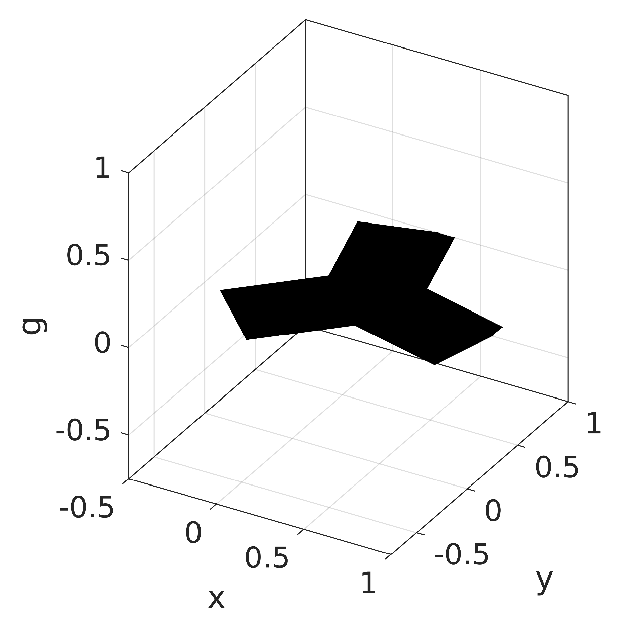
\includegraphics[width=1\linewidth]{./fig/moment_hull_1}
    \caption{}
  \end{subfigure}
  \begin{subfigure}[b]{0.24\textwidth}
    \centering
    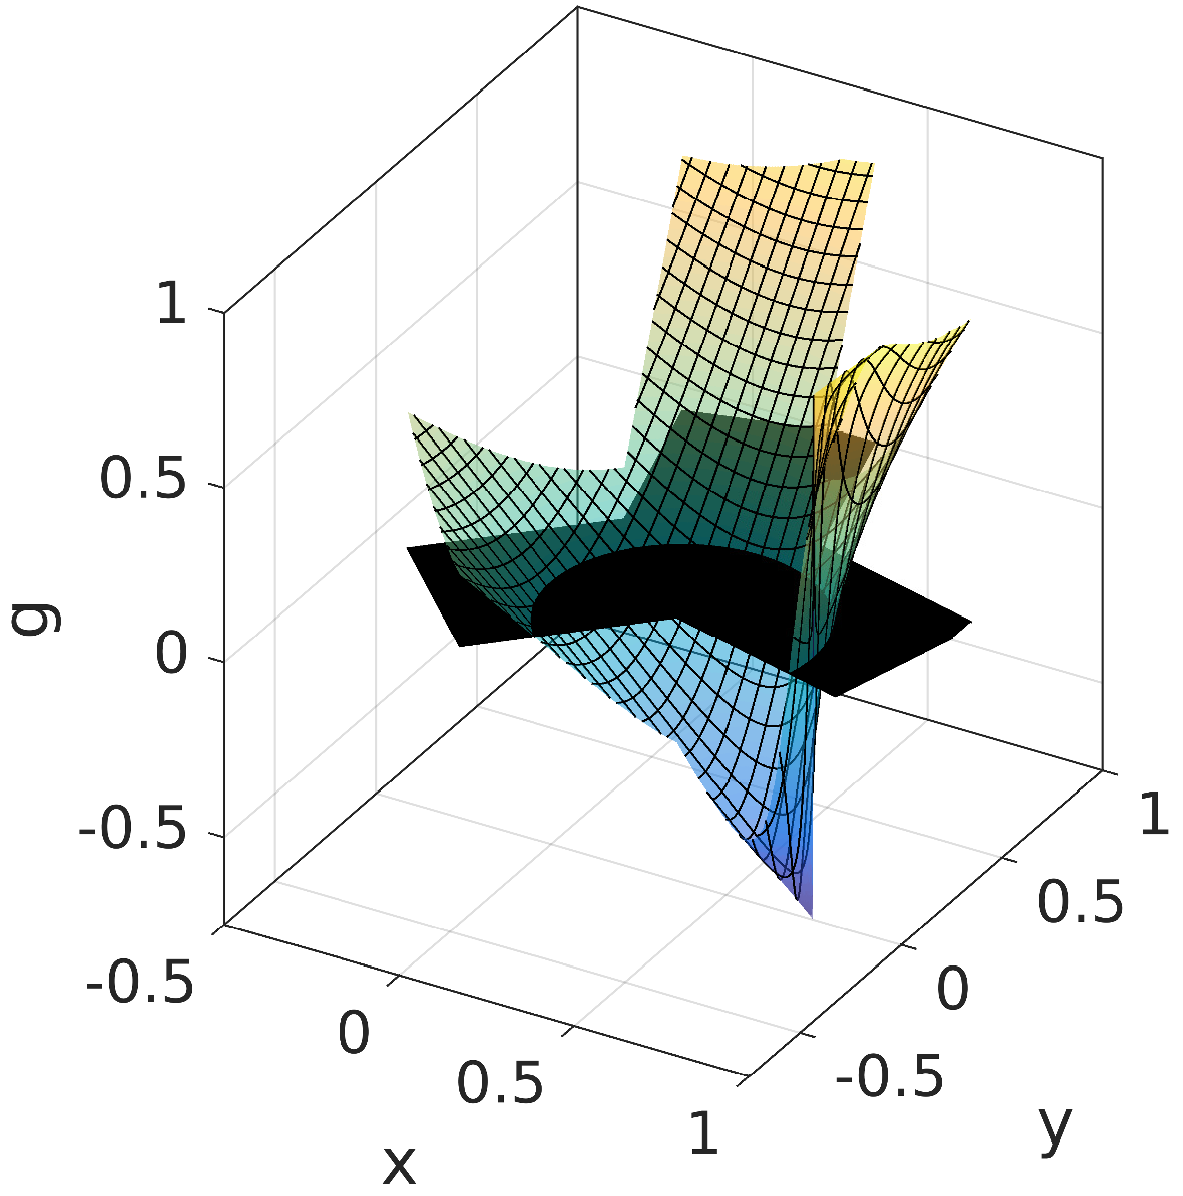
\includegraphics[width=1\linewidth]{fig/moment_hull_2}
    \caption{}
  \end{subfigure}
  \begin{subfigure}[b]{0.24\textwidth}
    \centering
    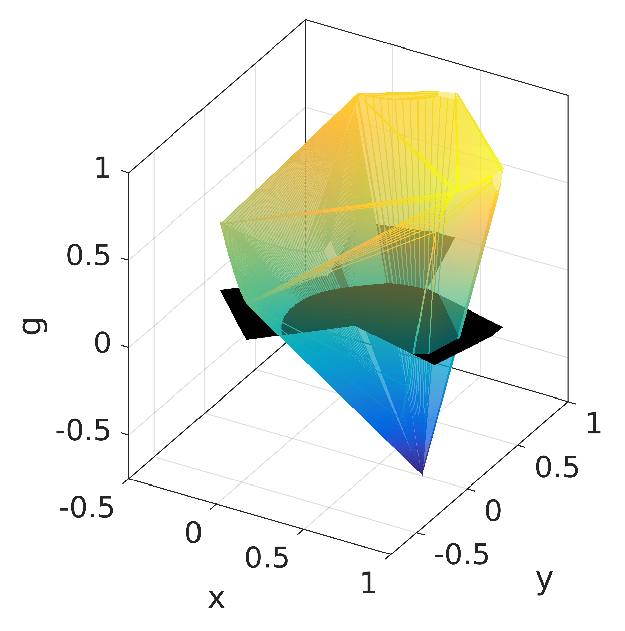
\includegraphics[width=1\linewidth]{fig/moment_hull_3}
    \caption{}
  \end{subfigure}
  \begin{subfigure}[b]{0.24\textwidth}
    \centering
    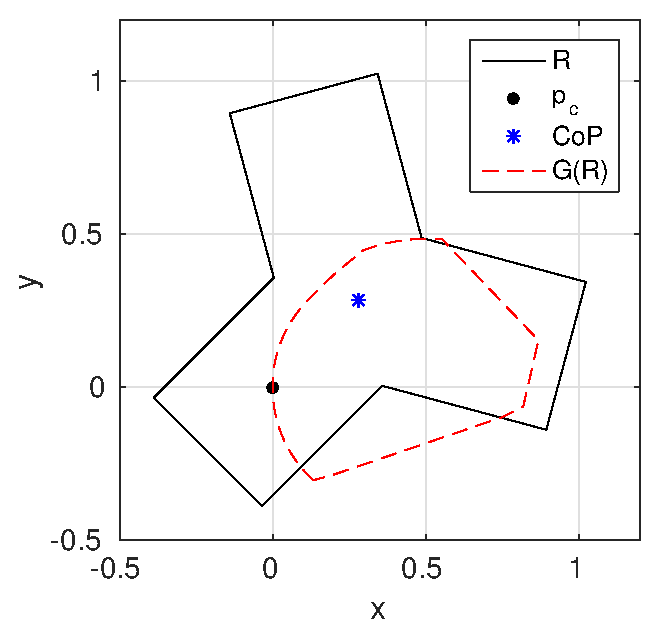
\includegraphics[width=1\linewidth]{fig/CoP_boundary}
    \caption{}
  \end{subfigure}
  \caption{Example moment envelope for a trigonal 2D object with
    rotation center $x_{\text{IC}} = 0.75$. (a) Support region
    $R$. (b) Normalized-moment surface $G(R)$. (c) Convex moment
    envelope of $G(R)$. (d) Intersection of the moment envelope and
    the $xy$-plane. The intersection bounds the set of feasible
    centers of pressure with zero moment.}
  \label{fig:moment-envelope}
\end{figure}

% \EH{TODO: Remove force hull}

The frictional moment envelope provides a nice geometric model of the
constraints between the center of pressure and moment at the contact
point \cite{Mason}. In this subsection, we show that the moment
envelope is important because it reduces the feasibility test of a
particular angular velocity to a point-in-convex-hull test.
% \EH{Add explanation of what this is used for later}
An example frictional moment envelope is illustrated step-by-step in
Figure \ref{fig:moment-envelope}.

A frictional moment envelope has as its parameters the support region
$R$ and twist $\mathbf{v}^+$. Let $f_0$ be the total normal
force. Then the function
\begin{equation}
  g(\mathbf{x}) = -\mu f_0\,\mathbf{x}\times \frac{A(\mathbf{x})\mathbf{v}^+}{\lVert A(\mathbf{x})\mathbf{v}^+ \rVert} \label{eq:unit-moment-at-x}
\end{equation}
evaluates the frictional torque that would result from a unit
normalized pressure at $\mathbf{x}$. Let $G$ map $R$ into a surface in
$\mathbb{R}^3$ by associating each point $\mathbf{x} \in R$ with its
maximum potential moment $g(\mathbf{x})$, i.e.
\begin{equation}
G(\mathbf{x}) =
\begin{bmatrix*}
  x\\
  y\\
  g(\mathbf{x})
\end{bmatrix*}, \label{eq:moment-surface-function}
\end{equation}
and let $\hat{p} = p/f_0$ be the normalized pressure. Then the set
$\{\int_RG(\mathbf{r})\hat{p}(\mathbf{r})dA
\,|\int_R\hat{p}(\mathbf{r})dA=1 \}$
is the convex hull of the surface $G(R)$. Moreover, any point in the
convex hull of $G(R)$ satisfies
\begin{align*}
  \int_R G(\mathbf{r}) \hat{p}(\mathbf{r})dA &= \int_R 
  \begin{bmatrix*}
    x\\
    y\\
    g(\mathbf{x})
  \end{bmatrix*}
  \hat{p}(\mathbf{r})dA\\
  &= 
    \begin{bmatrix*}
      x_0\\
      y_0\\
      \int_R g(\mathbf{x}) \hat{p}(\mathbf{r})dA
    \end{bmatrix*}. \numberthis
\end{align*}
Thus, the convex hull of $G(R)$ is the set of all feasible centers of
pressure and frictional moments for a given support region $R$ and
twist $\mathbf{v}^+$. We refer to the convex hull of $G(R)$ as the
\textit{moment envelope generated by $\mathbf{v}^+$}.  Therefore,
given a center of pressure $[x_0,y_0]^T$, an angular velocity $\omega$
is feasible if and only if the point $[x_0,y_0,0]^T$ is contained in
the moment envelope generated by $\omega$.

\section{Theory}\label{sec:theory}

This section covers our theoretical contributions. Subsection
\ref{sec:stable-equil-when} proves the existence and uniqueness of the
stable equilibrium during pulling. This result motivates our main
contributions. Subsection \ref{sec:prop-angular-velocity-bounds} lays
the theoretical groundwork necessary for proving the correctness of
the exact angular velocity bound algorithm introduced in
\ref{sec:exact-ang-vel-bound-alg}. Subsection
\ref{sec:orientation-bounds} extends the angular velocity bounds to
orientation bounds. This subsection completes the theoretical tools
needed in Subsection \ref{sec:diff-dynam-progr} to generate robotic
pulling trajectories that guarantee convergence to the final pose.

% to guarantee convergence of the
% robotic pulling trajectories generated in Subsection
% \ref{sec:diff-dynam-progr}.

% plan robotic pulling trajectories with
% convergence guarantees (Subsection \ref{sec:diff-dynam-progr}).
% These last two subsections build the machinery needed to plan robotic
% pulling trajectories with convergence guarantees (Subsection
% \ref{sec:diff-dynam-progr}).
% Lastly, \ref{sec:stability} contains a proof of
% the existence and uniqueness (modulo $2\pi$) of a stable equilibrium
% when pulling an object.

\subsection{Stable Equilibrium When Pulling}\label{sec:stable-equil-when}

For completeness, we prove the existence and uniqueness of the stable
equilibrium that occurs when pulling a rigid body. The existence of
the stable equilibrium was observed, without proof, in Mason
\cite{mason1986}, Lynch and Mason \cite{lynch1995pulling}, and
Berretty et al. \cite{berretty2001orienting}. The robotic pulling
trajectories generated in Subsection \ref{sec:diff-dynam-progr}
automatically use the stable equilibrium to reduce pose uncertainty.

\begin{theorem} \label{thm:cop-lom-convergence}
  For pulling of a rigid body in the plane, the rigid body converges
  to the state where its center of pressure is collinear with the
  pulling direction.
\end{theorem}

\begin{proof}
  We know from Theorem 7.4 in \cite{Mason} that the rigid body
  translates when the center of pressure is already collinear with the
  pulling direction. Now, suppose the center of pressure is strictly
  to the right of the pulling direction (as in Figure
  \ref{fig:presspull-motion}). Then by Theorem 7.4 in \cite{Mason},
  the rigid body rotates clockwise about the contact point, i.e. has
  angular velocity $\omega < 0$. Let $\varphi \in (\pi, 0)$ be the
  angular deviation of the rigid body. Since $\varphi$ is
  monotonically decreasing and $\omega = 0$ if $\varphi = 0$, we see
  that $\varphi$ converges to $0$ in the limit as
  $t \rightarrow \infty$. The case when the center of pressure is
  strictly to the left of the line of motion follows from symmetry.
  % When the line of motion passes through the center of pressure,
  % a pure translation takes place (Theorem 7.4 in \cite{Mason}). This
  % implies that $\dot{\theta} = 0$ if and only if
  % $\theta = \pi/2, -\pi/2$. Since $\theta$ is monotonically
  % decreasing, we see that it must converge to $-\pi/2$ in the limit as
  % $t \rightarrow \infty$.
  % Let the $y$-axis of the coordinate frame be aligned with the line of
  % motion of the press-pull contact point (see Figure
  % \ref{fig:presspull-motion} for an example). Then the instantaneous
  % rotation center of the body must fall on the $x$-axis, and we can
  % write $\mathbf{r}_\text{IC} = (x_\text{IC},0)^T$.
  % Suppose the center of pressure is strictly to the right of the line
  % of motion (as in Figure \ref{fig:presspull-motion}). Then by Theorem
  % 7.4 in \cite{Mason}, the rotation center lies on the positive
  % $x$-axis and has negative rotation. The velocity of a point on the
  % rigid body is given by
  % $\mathbf{v}(\mathbf{r}) =
  % \dot{\theta}\,\hat{\mathbf{k}}\times(\mathbf{r} -
  % \mathbf{r}_\text{IC})$.
  % We can compute the motion of the body relative to the contact point
  % by
  % \begin{align*}
  %   \mathbf{v}(\mathbf{r}) - \mathbf{v}_c &= \dot{\theta}\,\hat{\mathbf{k}}\times(\mathbf{r} - \mathbf{r}_\text{IC}) - \dot{\theta}\,\hat{\mathbf{k}}\times(\mathbf{0} - \mathbf{r}_\text{IC}) \\
  %   &= \dot{\theta}\,\hat{\mathbf{k}}\times(\mathbf{r} - \mathbf{0}) \numberthis \label{eqn:rel-rotation-center},
  % \end{align*}
  % where $\mathbf{v}_c$ is the velocity of the contact point. In other
  % words, the body is rotating clockwise relative to the
  % contact point with angular velocity
  % \begin{equation}
  %   \dot{\theta} = -\frac{\lVert\mathbf{v}_c\rVert}{x_\text{IC}}.
  % \end{equation}
  % Let $\theta \in (\pi/2, -\pi/2)$ be the orientation of the center of
  % pressure in the frame of the contact point. When the line of motion
  % passes through the center of pressure, a pure translation takes
  % place (Theorem 7.4 in \cite{Mason}). This implies that
  % $\dot{\theta} = 0$ if and only if $\theta = \pi/2, -\pi/2$. Since
  % $\theta$ is monotonically decreasing, we see that it must converge
  % to $-\pi/2$ in the limit as $t \rightarrow \infty$.
\end{proof}

\subsection{Properties of Angular Velocities Bounds}\label{sec:prop-angular-velocity-bounds}

% \EH{Comment: First proposition probably very unnecessary. Removable or
%   shortened.}
% \begin{proposition}
%   The constrained frictional dissipation equation
%   $\mathrm{D}_{\mathcal{C}}(\mathbf{v}^+)$ has a unique minimizer for
%   pressure distributions with some support force off of the
%   $x$-axis. When otherwise, the equation admits an interval of
%   minimizers.
% \end{proposition}

% \begin{proof}
%   The work of \cite{Mason1982} was the first to prove the above
%   observation for finite pressure distributions. For the case of
%   infinite (discrete) pressure distributions, we can appeal to the
%   convexity properties of $\lVert A(\mathbf{x})\mathbf{v}^+ \rVert$.

%   Minkowski's inequality gives
%   $\lVert x + y \rVert \leq \lVert x \rVert + \lVert y \rVert$ with
%   equality if and only if $x$ and $y$ are positively linearly
%   dependent. For two generalized velocities
%   $\mathbf{v}^+_1,\mathbf{v}^+_2\in \mathcal{C}$, the resulting body
%   point velocities are linearly dependent if and only if the
%   determinant
%   \begin{align}
%     \det A(\mathbf{x})
%       \begin{bmatrix*}
%         \mathbf{v}^+_1 & \mathbf{v}^+_2
%       \end{bmatrix*}
%     &= \det
%      \begin{bmatrix*}
%        -x_2\omega_1 & -x_2\omega_2 \\
%        1 + x_1\omega_1 & 1 + x_1\omega_2 
%      \end{bmatrix*}\\
%     &= -x_2(\omega_1 - \omega_2)
%   \end{align}
%   is zero. We immediately see that
%   $\lVert A(\mathbf{x})\mathbf{v}^+ \rVert$ is strictly convex
%   relative to $\mathcal{C}$ if and only if the body point $\mathbf{x}$
%   lies off of the $x$-axis. The proposition follows from the fact that
%   the positive sum of convex functions and a strictly convex function
%   is strictly convex.
% \end{proof}

% An object whose contact region is two discrete points, e.g. a spoon,
% can have multiple minimizing angular velocities when aligned with the
% $x$-axis.

We prove that the set of feasible angular velocities for an object
with known center of pressure is connected and bounded. These two
properties justify the use of a bisection search to locate the minimum
and maximum angular velocities in Subsection
\ref{sec:exact-ang-vel-bound-alg}.

We begin by citing a proposition from variational analysis used in our
proofs of the main results.
\begin{proposition}\label{prop:var-analysis}
  Suppose $P(u) := \argmin_x f(x,u)$ with
  $f:\mathcal{X}\times\mathcal{U}\rightarrow\mathbb{R}$ continuous and
  level-bounded in $x$ locally uniformly in $u$. Then the set-valued
  mapping $P(u)$ is outer-semicontinuous and locally bounded.
\end{proposition}

\begin{proof}
  Proposition adapted from Corollary 7.42 and Theorem 1.17 in
  \cite{Rockafellar}.
\end{proof}

\begin{theorem}\label{thm:angular-velocities}
  For pulling of a planar rigid body with known center of pressure,
  the set of all feasible angular velocities is connected.
\end{theorem}

\begin{proof}
  Let $\Omega$ be the set of feasible angular velocities,
  w.r.t. (\ref{eq:constrained-frictional-dissipation}), for a given
  support region $R$ with known center of pressure. Suppose $\Omega$
  is non-empty.
  % $\Omega$ is nonempty since a single support point located at the
  % center of pressure has an analytic solution.
  Let $\omega_1, \omega_2 \in \Omega$ and let $p_1, p_2$ be their
  corresponding pressure distributions. Then the new distribution
  $p_t = tp_1 + (1-t)p_2$, with $t \in [0,1]$, shares the same center
  of pressure as $p_1,p_2$. Define the function
  \begin{equation}
    f(\omega, t) = \mu\int_R\lVert A(\mathbf{r})\mathbf{v}^+(\omega)\rVert p_t(\mathbf{r})dA,
  \end{equation}
  where $\mathbf{v}^+: \omega \rightarrow [0,1,\omega]^T$ and
  $\dom f:= \mathbb{R}\times[0,1]$. By inspection, $f$ is
  continuous. For all $t \in [0,1]$ and $\alpha \in \mathbb{R}$, the
  set $\{(\omega,t)\;|\;f(\omega,t)\leq \alpha\}$ is bounded because
  $f \rightarrow \infty$ as $|x|\rightarrow \infty$. Hence, $f$ is
  level-bounded in $\omega$ locally uniformly in $t$, and $f$
  satisfies the conditions of Proposition \ref{prop:var-analysis}.

  The image of a connected set by an outer-semicontinuous set-valued
  mapping whose values are nonempty and connected is connected
  \cite{hiriart1985images}. Let $P(t) := \argmin_\omega f(\omega,t)$.
  For a given $t$, the set $P(t)$ is convex-valued and therefore
  connected. Since $f$ is continuous and level-bounded, the set is
  also nonempty (Theorem 1.9 \cite{Rockafellar}). Therefore, the image
  $P([0,1])$ contains the interval connecting $\omega_1$ and
  $\omega_2$. Because the choice of $\omega_1,\omega_2$ was arbitrary,
  $\Omega$ is connected.
\end{proof}

In general, Theorem \ref{thm:angular-velocities} holds for any convex
set of pressure distributions with known center of pressure. 

% Note, the set of pressure
% distributions with identical centers of pressure is convex.

\begin{corollary}\label{cor:bounded}
  For pulling of a planar rigid body with known center of pressure,
  the set of all feasible angular velocities is bounded.
\end{corollary}

\begin{proof}
  We prove Corollary \ref{cor:bounded} separately for the cases when
  the rigid body's center of pressure lies strictly in the right-half
  plane, left-half plane, or on the $y$-axis.

  Suppose the center of pressure lies in the right-half plane of the
  contact frame. Then by Theorem 7.4 of \cite{Mason} the angular
  velocity of the pulled body is strictly negative and hence, $0$
  bounds $\Omega$ from above. To establish a lower bound, we appeal to
  the following two properties about the set of feasible rotation
  centers when pushing or pulling with sticking contact. First, the
  rotation center must lie on the $x$-axis. Second, the rotation
  center must lie behind the line bisecting the contact point and the
  center of pressure \cite{Mason}. We observe that any feasible
  rotation center must have the form $[x,0]$ with $x > x^* > 0$, where
  $x^*$ is the intersection of the bisecting line and the
  $x$-axis. Recall that, by convention, we fix the contact point
  velocity to $\mathbf{v}_c = [0,1]^T$. We compute the angular
  velocity $\omega^*$ at $[0,x^*]$ using $\mathbf{v}_c$ and see that
  $\Omega$ is bounded from below by
  \begin{equation}
    % \omega = -\frac{\lVert\mathbf{v}_c\rVert}{x} > -\frac{\lVert\mathbf{v}_c\rVert}{x^*}
    \omega^* = -\frac{\lVert\mathbf{v}_c\rVert}{x^*}.% < \omega, \quad \forall \omega \in \Omega
  \end{equation}
  Thus, $\Omega$ is bounded. The case when the center of pressure lies
  in the left-half plane follows from a symmetrical argument.  

  When the center of pressure is collinear with the pulling direction,
  the rigid body translates and $\Omega = \{0\}$ \cite{Mason}.
%   The angular velocity of the rotation centers is bounded by
%   We convert the rotation center into a twist in our coordinate frame
%   Given a contact point velocity $\mathbf{v}_c$,
%   We convert the rotation
%   center bound into twist space 
%   % \begin{equation}
%   % \end{equation}
% Let $x^* > 0$ be the intersection of 
%   We see that $\Omega$ is bounded below when we convert the rotation
%   center to angular velocity using
%   \begin{equation}
%     \omega^* = -\frac{\lVert\mathbf{v}_c\rVert}{x^*}, \label{eq:rot-to-ang}
%   \end{equation}
%   where the rotation center $x^*$, strictly positive, is the
%   intersection of the bisector line and the $x$-axis. Therefore,
%   $\Omega$ is bounded. The case when the center of pressure lies in
%   the left-half plane follows from a symmetrical argument.
% To establish a lower bound, we will use the Bisector Bound
%   which states that that the set of feasible rotation centers falls
%   behind the line bisecting the contact point and the center of
%   pressure \cite{Mason}.
  % By Theorem 7.4 of \cite{Mason}, the angular velocity of the body is
  % strictly negative when the center of pressure falls strictly in the
  % right half-plane. This shows that $\Omega$ is bounded above by
  % $\omega = 0$. The Bisector Bound \cite{Mason} states that the set of
  % feasible rotation centers falls behind the line bisecting the
  % contact point and the center of pressure. With respect to our
  % coordinate frame (Subsection \ref{sec:plan-push-subj}), we see that
  % $\Omega$ is bounded above when we convert the rotation center to
  % angular velocity using
  % \begin{equation}
  %   \omega^* = -\frac{\lVert\mathbf{v}_c\rVert}{x^*}, \label{eq:rot-to-ang}
  % \end{equation}
  % where the rotation center $x^*$, strictly positive, is the
  % intersection of the bisector line and the $x$-axis. Therefore,
  % $\Omega$ is bounded.
\end{proof}

\subsection{Integrated Orientation Bounds}\label{sec:orientation-bounds}

\begin{figure}[t]
  \centering
    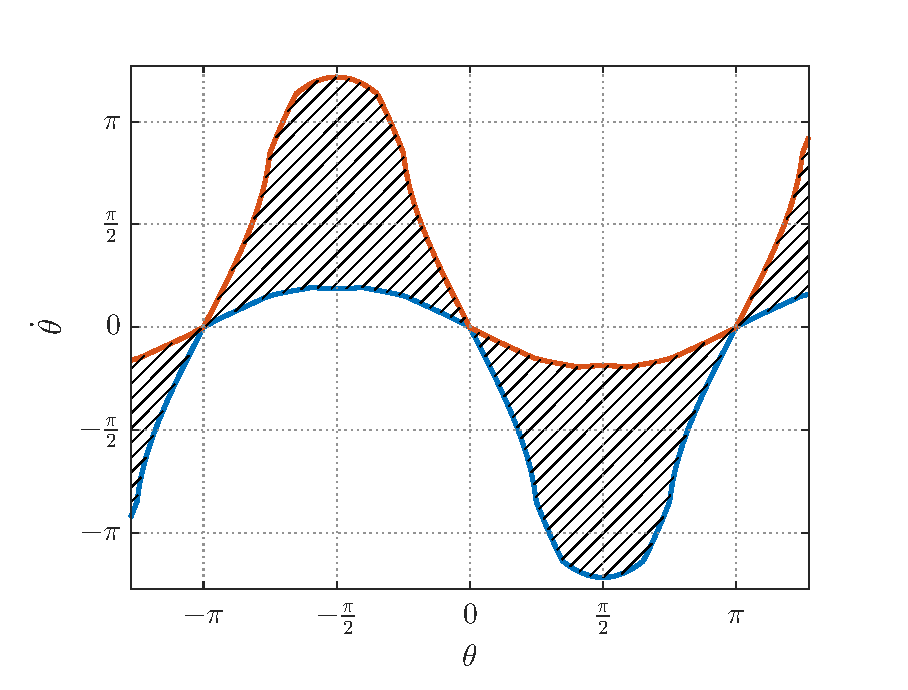
\includegraphics[width=1\linewidth]{fig/omega_bounds_1}
    \caption{Example angular velocity bounds for the trigonal 2D object from Figure \ref{fig:moment-envelope}. The object is oriented such that the stable pulling configuration corresponds to $\theta=0$. The orange curve is the upper bound $\alpha$. The blue curve is the lower bound $\beta$.}
  \label{fig:omega-bounds}
\end{figure}

We prove that the angular velocity bounds derived in Subsection
\ref{sec:prop-angular-velocity-bounds} integrate into bounds on the
orientation of the pulled body.

Let $\theta$ be the orientation of the rigid body in the world frame
and let $u$ and $l$ be upper and lower bounds on the orientation in
the world frame. Let the function $\omega(\rho)$ map from the angular
deviation to the angular velocity of the rigid body. Likewise, let the
functions $\alpha(\rho)$ and $\beta(\rho)$ map from the angular
deviation to the upper and lower angular velocity bounds.  An example
phase-plot of $\alpha(\rho)$ and $\beta(\rho)$ is illustrated in
Figure \ref{fig:omega-bounds}. Note the stable equilibrium at
$\theta = 0$.

% Likewise, let $u$ and $l$ be upper and lower bounds on the true
% orientation, and let the functions $\alpha$ and $\beta$ map from the
% angular deviation to the upper and lower angular velocity bound. 

We assume that the pulling trajectory
$\gamma:\mathbb{R}\rightarrow\mathbb{R}^2$ can be approximated by a
finite number of straight line segments of equal length. Given such a
$\gamma$, the pulling angle
$\phi(t) = \tan^{-1}(\dot{\gamma}_y(t),\dot{\gamma}_x(t))$ is a
piece-wise constant (step) function. Let
$v(t) = \lVert\dot{\gamma}(t)\rVert$. As the planar rigid body is
pulled along $\gamma$ with unit velocity, the state and bounds change
according to the dynamical system
\begin{align}
  \dot{x} &= \cos(\phi(t))\\
  \dot{y} &= \sin(\phi(t))\\
  \dot{\theta} &= \omega(\theta - \phi(t) + \pi)\\
  \dot{u} &=  \alpha(u - \phi(t) + \pi) \label{eq:u-ode}\\ 
  \dot{\ell} &=  \beta(\ell - \phi(t) + \pi)
\end{align}
where the expression $x - \phi(t) + \pi$ maps an orientation $x$ in
the global frame to the angular deviation.

\begin{proposition}\label{prop:orientation-bounds}
  For pulling of a rigid body with known initial pose, the orientation
  of the body is bounded above and below by $u$ and $\ell$.
\end{proposition}

\begin{proof}
  Suppose the proposition is false and $\theta$ crosses the bound $u$
  at time $t_0$, i.e. $u(t_0)=\theta(t_0)$ and $\theta(t) > u(t)$
  immediately afterwards. Let the line segment of $\gamma$ at $t_0$ be
  indexed by $i$ and have length $\varepsilon$. Then $\phi(t)$ is
  constant for $t$ in the range $[t_0,(i+1)\varepsilon)$. Pick $t_1$
  from said range such that $\theta(t_1) > u(t_1)$. Because $\phi$ is
  constant in $[t_0,t_1]$, we can apply separation of variables to
  solve differential equation (\ref{eq:u-ode}) and get
  \begin{equation}
    \int_{u(t_0)}^{u(t_1)}\frac{1}{\alpha(x - \phi(t_0))}dx = \int_{t_0}^{t_1}dt.
  \end{equation}
  This result shows that we can integrate the inverse of an angular
  velocity function to compute the amount of time required to reach a
  particular orientation. However, we can also apply separation of
  variables to the function $\omega$. Observe that because $\alpha$ is
  an upper bound on $\omega$
  \begin{equation} 
    \alpha(x - \phi(t_0)) \geq \omega(x - \phi(t_0)),
  \end{equation}
  the resulting integral of $\omega$ satisfies
  \begin{equation}
    \int_{u(t_0)}^{u(t_1)}\frac{1}{\alpha(x - \phi(t_0))}dx \leq \int_{u(t_0)}^{u(t_1)}\frac{1}{\omega(x - \phi(t_0))}dx.
  \end{equation}
  This indicates that $\theta(t_1) \leq u(t_1)$, a
  contradiction. Therefore, the upper bound holds and the lower bound
  follows from an identical argument.
\end{proof}

% \begin{proposition}
%   The angular velocity bounds on the motion of the pulled body are
%   continuous with respect to the orientation.
% \end{proposition}

% \begin{proof}
%   \TODO{
%     Sketch of proof idea:
%     \begin{enumerate}
%     \item A sequence of continuous functions which converges uniformly
%       to the lower bound $\alpha$ $\Rightarrow$ $\alpha$ is
%       continuous.
%     \item To construct such a sequence:
%     \item For all $N\in\mathcal{N}$, take $N$ evenly spaced points in
%       $[-\pi,\pi]$.
%     \item Can construct continuous function that approximates $\alpha$
%       by picking a minimum generating pressure distribution for each
%       $\theta_i$ and interpolating continuously between each
%       $\alpha(\theta_i)$.
%     \item If we can show the interpolating function has bounded
%       subgradient, then we can show it converges uniformly to
%       $\alpha$.
%     \item Intuitively we should be able to pick pressures $p_i$ and
%       $p_{i+1}$ for orientations $\theta_i$ and $\theta_{i+1}$ such
%       that they are ``close'' together. Then we need to show that
%       $p_i$ and $p_{i+1}$ being close implies that their minimizing
%       angular velocities are close in a global sense.
%     \item ?????
%     \end{enumerate}
%   }
% \end{proof}

% \subsection{Quasi-static Stability}\label{sec:stability}

% \EH{TODO: Simplify proof. Should be like two lines. It kind of makes
% the paper more schizophrenic, so might even remove it.}

% Note that the above proof holds for \textit{all pressure
%   distributions} of the body on the support
% surface.

\section{Methods}\label{sec:methods}

In this section, we synthesize the materials in Sections
\ref{sec:background} and \ref{sec:theory} into an algorithm for
computing exact angular velocity bounds and a method for planning
convergent trajectories using the computed bounds. The former is
detailed in Subsection \ref{sec:exact-ang-vel-bound-alg} and extended
in Subsection \ref{sec:point-in-moment-enve} and the latter is
detailed in Subsection \ref{sec:diff-dynam-progr}.

% The first subsection, \ref{sec:point-in-moment-enve}, details the
% changes to the moment hull (Subsection \ref{sec:frictional-envelope})
% that facilitate computations over a new class of pressure-distribution
% assumptions.

% Subsection \ref{sec:diff-dynam-progr} applies the exact angular
% velocity bounds to planning pulling trajectories using Differential
% Dynamic Programming (DDP).

\subsection{Exact Angular Velocity Bound
  Algorithm}\label{sec:exact-ang-vel-bound-alg}

\begin{algorithm}[t]
\caption{Exact Angular Velocity Bounds}\label{alg:angular-velocity-bounds}
\begin{algorithmic}[1]
\Function{Find Extrema}{$R$, $x_0$, $y_0$}
\If {$x_0$ is $0$} \Return {$[0,0]$}
\EndIf
% \BState \emph{min}:
\State $P \gets \min_\mathbf{x} \mathbf{0} \text{\;s.t.\;} R\mathbf{x} = [x_0,y_0]^T,  L \leq \mathbf{x} \leq U$ \label{line:find-pressure}
\State $x_r \gets \Call{Compute Rotation Center}{R,P}$ \label{line:find-rc}
\State $\omega \gets -\lVert\mathbf{v}_c\rVert/x_r$ \label{line:rc-to-w}
\State $l \gets 0$ \label{line:0}
\State $\omega_1 \gets \Call{Bisection Search}{R,x_0,y_0,l,\omega}$ \label{line:bisection-1}
% \BState \emph{max}:
\State $u \gets \omega$ \label{line:find-u-start}
\Do% {$u \gets 2u$}
\State {$u \gets 2u$} 
\State $\mathbf{v}^+ \gets [\mathbf{v}_c^T, u]^T$
\State $G \gets \{-\mathbf{x}\times A(\mathbf{x})\mathbf{v}^+ / \lVert A(\mathbf{x})\mathbf{v}^+ \rVert \;|\; \mathbf{x} \in R\}$
\DoWhile{$[x_0,y_0,0]^T \in \Call{ConvHull}{G}$} \label{line:find-u-end}
\State $\omega_2 \gets \Call{Bisection Search}{R,x_0,y_0,u,\omega}$ \label{line:bisection-2}
% \BState \emph{return}:
\State $l \gets \Call{Min}{\omega_1,\omega_2}$
\State $u \gets \Call{Max}{\omega_1,\omega_2}$
\State \Return {$[l, u]$}
\EndFunction
% 
\Function{Bisection Search}{$R$, $x_0$, $y_0$, $\alpha$, $\beta$}
\While{$\varepsilon < |\alpha-\beta|$}
\State $\omega \gets (\alpha + \beta)/2$
\State $\mathbf{v}^+ \gets [\mathbf{v}_c^T, \omega]^T$
\State $G \gets \{-\mathbf{x}\times A(\mathbf{x})\mathbf{v}^+ / \lVert A(\mathbf{x})\mathbf{v}^+ \rVert \;|\; \mathbf{x} \in R\}$
\If {$[x_0,y_0,0]^T \in \Call{ConvHull}{G}$} 
\State $\beta \gets \omega$
\Else{} 
\State $\alpha \gets \omega$
\EndIf
\EndWhile
\State \Return $(\alpha + \beta)/2$
\EndFunction
\end{algorithmic}
\end{algorithm}

% \EH{TODO: Explain correctness of algorithm using theoretical results}

Algorithm \ref{alg:angular-velocity-bounds} finds exact angular
velocity bounds for a given support region $R$ and center of pressure
$[x_0,y_0]^T$. It uses bisection search to estimate the end-points of
$\Omega$. This choice is justified because $\Omega$ is connected and
bounded by Theorem \ref{thm:angular-velocities} and Corollary
\ref{cor:bounded}.

To initialize the bisection search, we need an angular velocity in
$\Omega$ and two angular velocities above and below the bounds of
$\Omega$. First, we compute an angular velocity $\omega$ in $\Omega$.
We find a feasible assignment of pressures $P$ such that the center of
pressure is $[x_0, y_0]$ (line \ref{line:find-pressure}). From $P$,
the resultant rotation center $[x_r,0]$ can be computed using the
root-finding method in \cite{Mason1982} (line \ref{line:find-rc}).
Lastly, we convert the rotation center into the angular velocity
$\omega \in \Omega$ (line \ref{line:rc-to-w}). Of the two out-of-bound
angular velocities $l$ and $u$, we can set $l$ to $0$ (line
\ref{line:0}). The other can be found by repeatedly doubling $\omega$
until the resulting angular velocity is no longer feasible (lines
\ref{line:find-u-start}-\ref{line:find-u-end}). As a reminder, we test
the feasibility of a given angular velocity $\omega'$ by checking
whether the point $[x_0,y_0,0]^T$ is contained in the associated
frictional moment envelope (see Section
\ref{sec:frictional-envelope}). Now that $\omega$, $u$, and $l$ have
been computed, we pass them into the bisection search to compute the
boundary points of $\Omega$ (lines \ref{line:bisection-1} and
\ref{line:bisection-2}).

The run-time of the algorithm is $\mathcal{O}(d\,n\log{} n)$, where
$d$ is the number of significant digits returned and $n$ is the number
of points in the discretization of $R$. This computation is relatively
expensive to perform online. In Section \ref{sec:diff-dynam-progr}, we
avoid recomputing angular velocity bounds by fitting Fourier series to
a set of pre-computed orientation-bound pairs.

% To initialize, the bisection search first finds a feasible pressure
% distribution with center of pressure $[x_0,y_0]$ (line
% \ref{line:find-pressure}) and then finds a feasible rotation center
% using the root-finding method in \cite{Mason1982} (line
% \ref{line:find-rc}). The bisection search tests the feasibility of an
% angular velocity $\omega$ by checking whether the point
% $[x_0,y_0,0]^T$ is contained in the associated frictional moment
% envelope (see Section \ref{sec:frictional-envelope}).

% In quasi-static terminology, this is equivalent to checking whether
% there exists a pressure distribution with center of pressure
% $[x_0,y_0]^T$ such that the velocity
% $\mathbf{v}^+ = [\mathbf{v}_c^T, \omega]^T$ generates zero moment
% about the contact point (Equation \ref{eq:moment-at-contact}).

\subsection{Improving on Exact Angular Velocity Bounds}\label{sec:point-in-moment-enve}

% tightness of the bounds and the basic assumptions from which those
% bounds are deduced, such as knowledge of the center of pressure
% location.

The exact angular velocity bounds computed in Section
\ref{sec:exact-ang-vel-bound-alg} result in slow convergence towards
the stable pulling equilibrium point (for experimental measurements,
see Subsection \ref{sec:bound-comparison}). Consequently, wide bounds
cause our planner to generate long trajectories that exceed the
robot's workspace in order to satisfy tolerances on the final pose
uncertainty.

In this subsection, we show how to modify the constraints on the
pressure distributions from which the bounds were computed. This
allows us to restrict pressure distributions to smaller subclasses and
thus achieve tighter angular velocity bounds. Let $\mathcal{C}$ be the
class of normalized pressure distributions over a region $R$ with
center of pressure $[x_0, y_0]$.
% Note, as written, Algorithm
% \ref{alg:angular-velocity-bounds} checks the feasibility of an angular
% velocity with respect to $\mathcal{C}$.
Now, suppose we had a convex subclass $\mathcal{K}$ of pressure
distributions such that $\mathcal{K} \subset
\mathcal{C}$. Regrettably, the point-in-convex-hull feasibility test
only works for $\mathcal{C}$. However, we can setup an alternative
feasibility test with respect to $\mathcal{K}$ by solving the linear
program
\begin{equation}
  \begin{aligned}
    & \underset{p}{\text{minimize}}
    & & \left\lVert \sum_Rg(\mathbf{r})p(\mathbf{r})\right\rVert \\
    & \text{subject to} 
    & & p \in \mathcal{K}
  \end{aligned} \label{eq:lin-prog-feasibility}
\end{equation}
where $p$ is a discretized pressure distribution, $g(\mathbf{r})$ is
the unit-torque function from equation (\ref{eq:unit-moment-at-x}),
and the summation is over points $\mathbf{r} \in R$. A given angular
velocity $\omega$ is feasible if and only if the linear program
(\ref{eq:lin-prog-feasibility}) finds a pressure distribution $p$ such
that the objective
$\left\lVert \sum_Rg(\mathbf{r})p(\mathbf{r})\right\rVert$ is $0$ and
$p \in \mathcal{K}$.

Several options exists for the choice of $\mathcal{K}$. 
In our experiments, we use
\begin{equation}
  \mathcal{K} = \{p\;|\; 0 \leq p_i \leq U, p \in \mathcal{C}\} \label{eq:upper-bound-pressures}
\end{equation}
where $U \leq 1$ is an upper bound on the discretized pressures. The
upper bound $U$ controls the percentage of $R$ guaranteed to be in
contact with the surface, i.e. has non-zero pressure. For example, if
we set $U = 2/N$, where $N$ is the number of points in the
discretization of $R$, then, by the pigeon-hole principle, at least
50\% of $R$ is always in contact with the surface. Our implementation
solves linear program (\ref{eq:lin-prog-feasibility}) using
\texttt{Gurobi} \cite{gurobi}.

% The set (\ref{eq:upper-bound-pressures}) has the following physical
% interpretation. Set the upper bound $U$ to $2/N$, where $N$ is the
% number of points in the discretization of the contact region $R$. Then
% by the pigeon-hole principle, at least 50\% of $R$ is in contact with
% the surface.

% Let $N$ be the number of points in the discretization
% of the contact region $R$. Set $U$ to $2/N$. Then by the pigeon-hole
% principle, at least 50\% of $R$ is always in contact with the surface.


% The upper and lower bounds, $U$ and $L$, have a nice physical
% interpretation. Let $N$ be the number of points in the discretization
% of the contact region $R$. Set $U$ to $2/N$. Then by the pigeon-hole
% principle, at least 50\% the area of $R$ is always in contact with the
% surface.  Or set $L$ to $0.1/N$. Then at least 10\% of object weight
% is uniformly distributed.

% We know from Subsection \ref{sec:frictional-envelope} that we can test
% the feasibility of an angular velocity $\omega$ by querying whether
% the moment envelope generated by $\omega$ contains the point
% $[x_0,y_0,0]^T$, where $[x_0,y_0]^T$ is the object's center of
% pressure. Implicitly, this method checks feasibility against the class
% of pressure distributions with shared center of pressure. However,
% this assumption is often too broad in practice. We cast the
% feasibility test as a linear program to facilitate checking against
% new classes of pressure distributions, including, for example, bounds
% on the pressure magnitude at various points. 

% This linear program checks the feasibility of angular velocity by
% directly solving for an assignment of discrete, bounded pressures such
% that the pushed object has the correct center of pressure and
% generates zero moment
% \begin{equation}
%   \begin{aligned}
%     & \underset{\mathbf{p}}{\text{minimize}}
%     & & \mathbf{0} \\
%     & \text{subject to}
%     & & G\mathbf{p} = [x_0,y_0,0]^T,\; \mathbf{1}\cdot\mathbf{p} = 1, \\
%     & & & L \leq \mathbf{p} \leq U,
%   \end{aligned} \label{eq:lin-prog-PiCH}
% \end{equation}
% where $\mathbf{p}$ is a normalized pressure distribution, $G$ is the
% moment surface function (\ref{eq:moment-surface-function}) computed
% over the discretized support region $R$, and $L$ and $U$ are bounds on
% $\mathbf{p}$.

% The upper and lower bounds, $U$ and $L$, have a nice physical
% interpretation. Let $N$ be the number of points in the discretization
% of the contact region $R$. Set $U$ to $2/N$. Then by the pigeon-hole
% principle, at least 50\% the area of $R$ is always in contact with the
% surface.  Or set $L$ to $0.1/N$. Then at least 10\% of object weight
% is uniformly distributed.

% We solve the linear program (\ref{eq:lin-prog-PiCH}) using
% \texttt{Gurobi} \cite{gurobi}.

\subsection{Planning Convergent Trajectories for Robotic
  Pulling}\label{sec:diff-dynam-progr}
% \begin{inparaenum}
% \item contact point(s)
% \item initialization
% \item discretized dynamics
% \item cost functions
% \item Yifan's DDP code
% \item Which ddp algorithm was used
% \end{inparaenum}
% \EH{TODO: Tie in theoretical results on uncertainty into DDP} 

We use control-limited Differential Dynamic Programming (DDP)
\cite{tassa2014control} to plan trajectories for robotic pulling.  Our
implementation uses the following first order approximation of the
discretized dynamics
\begin{align}
  x_{i+1} &= x_i + d_i\cdot\cos(\phi_i) \\
  y_{i+1} &= y_i + d_i\cdot\sin(\phi_i)\\
  u_{i+1} &= u_i + d_i\cdot\hat{\alpha}(u_i - \phi_i + \pi) \\
  \ell_{i+1} &= \ell_i + d_i\cdot\hat{\beta}(\ell_i - \phi_i + \pi)\\
  h_{i+1} &= h_i + d_i.
\end{align}
In this system, the controls at index $i$ are the distance $d_i$ and
heading $\phi_i$. The functions $\hat{\alpha}$ and $\hat{\beta}$ are
Fourier series approximations of the upper and lower bounds $\alpha$
and $\beta$. The variable $h_i$ measures the cumulative distance
pulled.

Let $\mathbf{x}_i = [x_i,y_i,u_i,l_i]^T$ and
$\mathbf{u}_i = [d_i,\phi_i]^T$, with $i\in[1,N]$. In our DDP planner,
we set the running cost $\mathcal{L}(\mathbf{x}_i,\mathbf{u}_i)$ to
zero. We set the final cost to be
\begin{equation}
\mathcal{L}_F(\mathbf{x}_N,h_N) = \mathbf{k}^T\mathcal{L}_{\bm{\delta}}(\mathbf{x}_N-\mathbf{x}_F) + \lambda h_N^2,
\end{equation}
where $\mathcal{L}_{\bm{\delta}}$ is the vectorized version of the
Pseudo-Huber loss function \footnote{This function approximates an
  $\ell_1$ norm for $a > \delta$.}
\begin{equation}
\mathcal{L}_{\delta}(a) = \sqrt{a^2+\delta^2}-\delta,
\end{equation}
$\mathbf{x}_F$ is the goal configuration, $\mathbf{k}$ is the slope of
the vectorized Pseudo-Huber loss function, $\bm{\delta}$ is the width
of the vectorized Pseudo-Huber loss function, and $\lambda$ is the
distance penalty coefficient. We set the final upper and lower bounds,
$u_N$ and $\ell_N$, to be equal in the target state
$\mathbf{x}_F$. This ensures the generated trajectory converges
towards the target orientation (due to Proposition
\ref{prop:orientation-bounds}).

We initialize our optimizer using paths generated from Dubin's curves
\cite{dubins1957curves} because pulling with sticking contact shares
similar dynamics with the simple car \cite{lavalle1999planning}.
Dubin's curves are time-optimal paths for simple cars. The curves
consist of constant curvature turns and straight line segments. To
apply these curves to our system, we need two pieces of information:
the minimum turning radius and the effective rear axle center. 

Given a heading $\omega \in (0,\pi/2) $ and resulting upper angular
velocity bound $\alpha(\omega)$ in the frame of the contact point, the
minimum turning radius is equivalent to the distance from the center
of rotation to the line between the contact point and the center of
pressure $\mathbf{p}_0 = [x_0,y_0]^T$, that is
\begin{equation}
  r_{\text{min}} = \frac{\sign y_0}{\alpha(\omega)},
\end{equation}
and the effective rear axle center is the projection of the rotation center onto that line, i.e.
\begin{equation}
  \mathbf{c}_{\text{rear}} = -\frac{x_0}{\alpha(\omega)}\cdot\frac{\mathbf{p}_0}{\lVert \mathbf{p}_0 \rVert^2}.
\end{equation}
% From these, we can compute Dubin's curves for our initialization.


\section{Experiments}\label{sec:experiments}
% \EH{Spin the experiments: We chose experiments that underscore the
%   practical benefits of our theoretical contributions.}

\subsection{Comparison of
  Angular Velocity Bounds}\label{sec:bound-comparison}

In this experiment, we compare distance-to-convergence for our exact
angular velocity bounds and the previous best bound, i.e. the Peshkin
bound \cite{peshkin1988motion}. We test the bounds over the objects in
the MIT Pushing Dataset \cite{YuBFR16} and randomly generated bipods,
tripods, and quadrapods. The generated $n$-pods were chosen to have
circumcircle diameters similar to the MIT objects, roughly $0.16$m.

% \begin{inparaenum}
% \item MIT objects
% \item Generated 30 random $n$-pods for each $n$
% \item We sampled $10$ contact points and computed distance to
%   convergence for each point.
% \end{inparaenum}

For each MIT object, we picked $10$ even spaced contact points on the
boundary of the object. We generated $30$ random $n$-pods for each
category and took the contact point to be the center of a random pod
(similar to pulling the leg of a chair). We compute
distance-to-convergence in the following manner. Let $\gamma$ be an
angular velocity bound (can be upper or lower). We orient the object
such that the center of pressure is 90 degrees away from the stable
configuration. Next, we simulate a pulling trajectory while
integrating $\gamma$ and stop when the integral converges to within 1
degree of the stable configuration. The distance travelled is the
distance-to-convergence\footnote{Note that this distance is
  independent of the pulling velocity, see Equation
  (\ref{eq:rot-to-ang}).}. 

The experimental results are collected in Table
\ref{table:convergence-distance}. 
% When interpreting the table, remember that an angular velocity bound
% $\gamma$ is, in general, not symmetric about the origin, that is
% $\gamma(\theta - \pi) \neq \gamma(\theta)$, and that $\gamma$ is
% negative when $\theta$ is 90 degrees (see Figure
% \ref{fig:omega-bounds}).
The Peshkin bound computes the feasible angular velocities for the
circumcircle enclosing the object. As a result, it underestimates the
slowest angular velocity bound and its distance-to-convergence can be
twice are far as compared to the exact bound.  When feasible pressure
distribution are restricted such that at least 50\% of the object is
in contact with the surface, the distance-to-convergence of the exact
bound is reduced by another factor of two. Because the exact bound
converges within $3/4$ a meter, it is serviceable for manipulating the
MIT objects on a large table. Naturally, smaller objects or tighter
bounds are required for smaller tables. 

\begin{table}[t]
  \begin{center}
      \begin{tabular}[c]{cccc}
        \toprule
        & Exact & Exact-50\% & Peshkin \\
        \midrule
        MIT & $\begin{matrix}0.670\\0.172\end{matrix} \begin{matrix}\pm\\\pm\end{matrix} \begin{matrix}0.141\\ 0.047\end{matrix}$ & $\begin{matrix}\mathbf{0.362}\\\mathbf{0.243}\end{matrix} \begin{matrix}\pm\\\pm\end{matrix} \begin{matrix}0.073\\ 0.053\end{matrix}$ & $\begin{matrix}1.354\\0.162\end{matrix} \begin{matrix}\pm\\\pm\end{matrix} \begin{matrix}0.501\\ 0.041\end{matrix}$ \\
        \midrule
        Bipod & $\begin{matrix}0.762\\0.516\end{matrix} \begin{matrix}\pm\\\pm\end{matrix} \begin{matrix}0.210\\ 0.218\end{matrix}$ & $\begin{matrix}\mathbf{0.692}\\\mathbf{0.574}\end{matrix} \begin{matrix}\pm\\\pm\end{matrix} \begin{matrix}0.213\\ 0.216\end{matrix}$ & $\begin{matrix}0.899\\0.273\end{matrix} \begin{matrix}\pm\\\pm\end{matrix} \begin{matrix}0.239\\0.095\end{matrix}$ \\
        \midrule
        Tripod & $\begin{matrix}0.765\\0.522\end{matrix} \begin{matrix}\pm\\\pm\end{matrix} \begin{matrix}0.133\\ 0.162\end{matrix}$ & $\begin{matrix}\mathbf{0.688}\\\mathbf{0.576}\end{matrix} \begin{matrix}\pm\\\pm\end{matrix} \begin{matrix}0.143\\ 0.157\end{matrix}$ & $\begin{matrix}1.180\\0.340\end{matrix} \begin{matrix}\pm\\\pm\end{matrix} \begin{matrix}0.244\\0.108\end{matrix}$ \\
        \midrule
        Quadrapod & $\begin{matrix}0.880\\0.417\end{matrix} \begin{matrix}\pm\\\pm\end{matrix} \begin{matrix}0.120\\ 0.099\end{matrix}$ & $\begin{matrix}\mathbf{0.749}\\\mathbf{0.489}\end{matrix} \begin{matrix}\pm\\\pm\end{matrix} \begin{matrix}0.114\\ 0.098\end{matrix}$ & $\begin{matrix}1.207\\0.329\end{matrix} \begin{matrix}\pm\\\pm\end{matrix} \begin{matrix}0.235\\0.096\end{matrix}$ \\
        \bottomrule
      \end{tabular}
  \end{center}
  \caption{Comparison of distance-to-convergence (in meters) for different objects and angular velocity bounds. The top and bottom values in each cell correspond to distances from the upper and lower angular velocity bounds, respectively. See Section \ref{sec:bound-comparison} for the experimental setup.}
  \label{table:convergence-distance}
\end{table}

\subsection{Robotic Pulling on a Tabletop}
\begin{figure}
  \begin{center}
    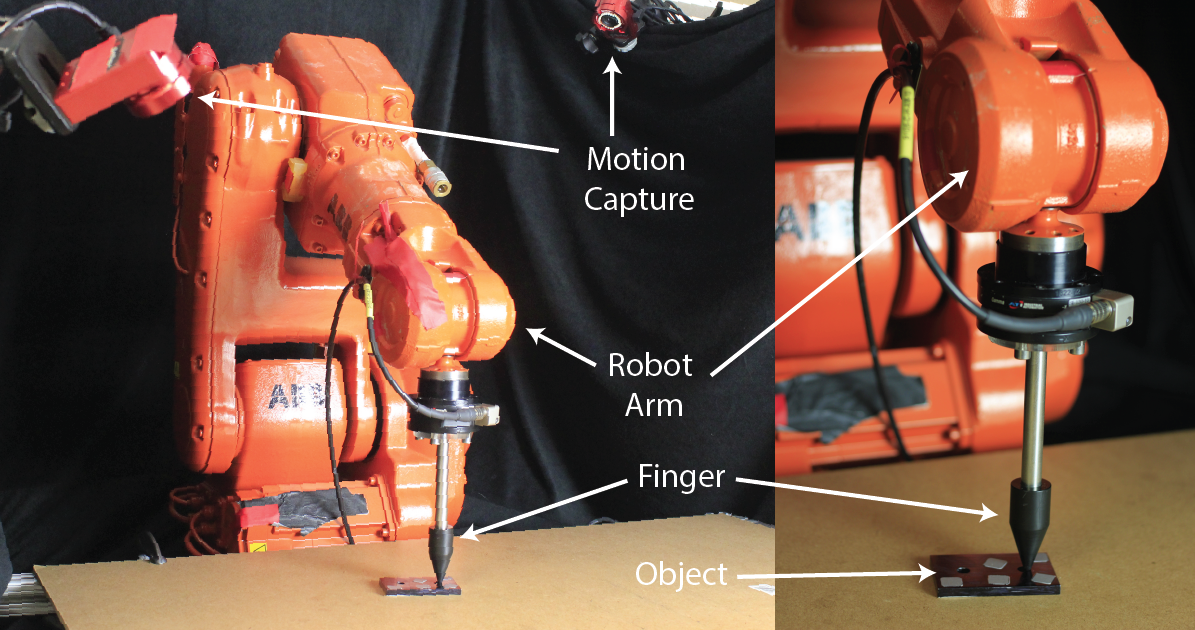
\includegraphics[width=\columnwidth]{fig/hardware.png}
  \end{center}
  \caption{Hardware setup for robotic pulling experiments.}
  \label{fig:hardware}
\end{figure}

Figure \ref{fig:hardware} shows the experimental setup that we used to
test the robotic pulling trajectories generated by the planning
algorithm in Subsection \ref{sec:diff-dynam-progr}.

% With this experiment we aim to test mainly two things:
% \begin{itemize}
% \item the validity of the trajectories generated by the planner, and
% \item convergence of the pulled object to the commanded pose.
% \end{itemize}

Experimental data was collected using an ABB 140 manipulator equipped
with a conical finger. The test object was a laser-cut acrylic
rectangle (75mmx50mmx6.35mm) with 8 holes at the edges and
corners. The conical finger moved the acrylic rectangle by pulling
inside the holes.  A 5 camera OptiTrack motion capture system was set
up to record ground truth position of the object in 2D with a accuracy
of 2mm. To compensate sensing error, the holes on the rectangle were
oversized to have a 3mm radius. We used MDF board as our surface
material.

\begin{figure}
\begin{center}
  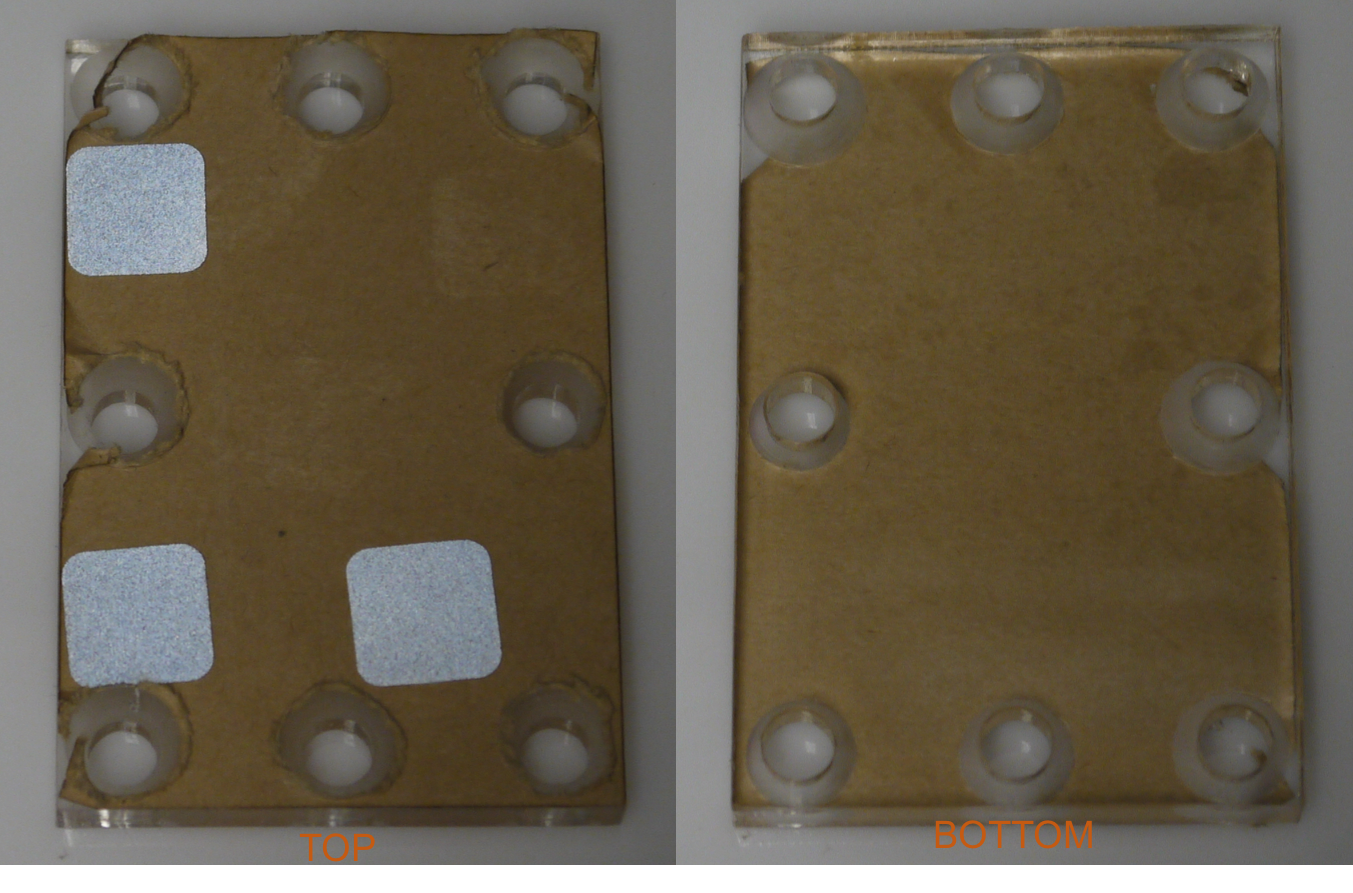
\includegraphics[width=\columnwidth]{fig/object}
\end{center}
\caption{The top and bottom view of the acrylic rectangle with motion
  capture markers and 8 holes for pulling.}
\label{fig:object}
\end{figure}

We computed angular velocity bounds for the acrylic rectangle over
pressure distributions restricted to have at least 25\% of the object
is in contact with the surface. The slope $\mathbf{k}$ of the
Pseudo-Huber Loss function for the DDP planner was set to
$[5000, 5000, 1000, 1000]$ and the width $\bm{\delta}$ was set to
$[0.01, 0.01, 0.02, 0.02]$. The distance penalty $\lambda$ was set to
$40$. For each pulling trial, we generated random start and end poses
within the vision system's field of view. The planner was evaluated
for all eight contact points and the lowest cost trajectory that
remained within the robot workspace was executed on the robot at
25mm/s linear speed. The final pose was then recorded by the motion
capture system.

We collected 80 trials of robotic pulling. Of those, we discarded the
4 trials where the algorithm failed to find any feasible trajectory
within the robot workspace. The average absolute displacement from the
target pose was 4.00mm $\pm$ 3.02mm. The average absolute angular
displacement from the target pose was 4.35 degrees $\pm$ 3.14
degrees. Note the hole radius introduces a systematic error of 3mm to
the final pose because the puller contacts the edge of the hole, not
the center. Overall, our experimental results support the claim that
the planner finds convergent pulling trajectories. An example trial is
visualized in Figure \ref{fig:trajectory}.

% We distinguish between two types of error during the pulling
% experiments. The target error is the error between the target pose and
% the final pose measured by the MoCap. The commanded error is the error
% between the last commanded pose and the final pose measured by the
% MoCap.

% This distinction is important because the target error quantifies the
% performance of our planner, while the commanded error quantifies the
% performance of our theoretical bounds.

% avg_radial_error =
%     0.0040
% std_radial_error =
%     0.0030
% avg_angular_error =
%     4.3457
% std_angular_error =
%     3.1450

% \begin{table}[t]
  % \begin{center}
  %     \begin{tabular}[c]{cccc}
  %       \toprule
  %       & $r$ & $\theta$ \\
  %       \midrule
  %       target & & & \\
  %       \midrule 
  %       command & & & \\
  %       \bottomrule
  %     \end{tabular}
  % \end{center}
  % \caption{Comparison of distance-to-convergence (in meters) for different objects and angular velocity bounds. The top and bottom values in each cell correspond to distances from the upper and lower angular velocity bounds, respectively. See Section \ref{sec:bound-comparison} for the experimental setup.}
% \end{table}

\begin{figure}
\begin{center}
  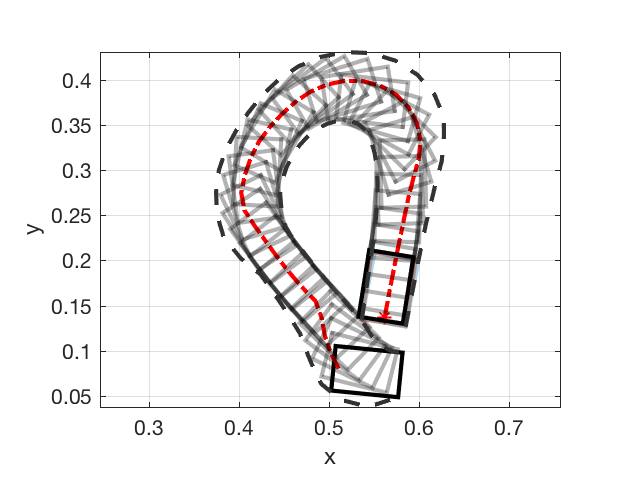
\includegraphics[width=\columnwidth]{fig/trajectory_2.eps}
\end{center}
\caption{(Dashed red line) The planned robotic pulling
  trajectory. (Dashed black line) The area swept by the possible poses
  computed by our bounds during the planned trajectory. (Grey
  rectangles) The measured poses of the object when the trajectory was
  executed on a real robot.}
\label{fig:trajectory}
\end{figure}

\section{Future Work}\label{sec:future work}
{
  \color{red}
  \begin{inparaenum}
  \item Extension of the proposed planner to general objects (increase the scope of the contribution).
  \item NAMO
  \item Press-pulling
  \item 
  \end{inparaenum}
}

% \section{Discussion}\label{sec:discussion}
\section{Conclusion}\label{sec:conclusion}

In this paper, we derive a method for computing exact bounds on the
object's motion for classes of pressure distributions where the center
of pressure is known but the distribution of support forces is
unknown. We also show these exact motion bounds can be used to plan
robotic pulling trajectories that guarantee the pulled object
converges to the final pose. We validate our planner on a real robotic
system and show that the generated trajectories obtain low errors on
the final pose of the object.

\bibliographystyle{plainnat}
\bibliography{references}

\end{document}


